\section{Prima parte - DCT2 benchmark}
\subsection{Obiettivo}
    In questa prima parte dell'elaborato si richiede di fornire una propria implementazione dell'algoritmo \textbf{\textit{DCT2} (Discrete Cosine Transform 2-dimensional)} in ambiente \textbf{open source} e di confrontare le performance ottenute (in termini di \textbf{tempo di esecuzione}) con un'implementazione fornita da una libreria dell'ambiente open source.
    
    A tal fine si è scelto di utilizzare il linguaggio di programmazione \textbf{python} e le librerie \href{https://docs.scipy.org/doc/scipy/}{\textbf{\textit{scipy}}}, dedicata al \textbf{calcolo scientifico}, e \href{https://numpy.org/}{\textbf{numpy}}, descritte nel dettaglio nel paragrafo \ref{subsec:library}.

    Successivamente, al fine di determinare l'impatto di implementazioni più o meno efficienti sui \textbf{tempi di esecuzione}, sono state fornite tre diverse implementazioni personali dell'algoritmo \textbf{\textit{DCT2}}, trattate nel paragrafo \ref{subsec:implementations}.

    Come indicato nelle specifiche, per semplicità verranno trattate solo matrici quadrate.

\subsection{Libreria} \label{subsec:library}
    La libreria \textbf{scipy} mette a disposizione il modulo \href{https://docs.scipy.org/doc/scipy/reference/fftpack.html}{\textbf{fftpack}}, contenente una serie di funzioni che permettono di calcolare diverse varianti della \textit{Discrete Cosine Transform}.

    In particolare, nella stesura di questo elaborato è stata utilizzata unicamente la funzione \href{https://docs.scipy.org/doc/scipy/reference/generated/scipy.fftpack.dctn.html#scipy.fftpack.dctn}{\textit{dctn}}, che permette di specificare uno o più assi lungo i quali eseguire la \textit{DCT}. Per ottenere lo \href{https://docs.scipy.org/doc/scipy/reference/generated/scipy.fftpack.dct.html#scipy.fftpack.dct}{scaling} indicato nel progetto sono stati usati i parametri:
    \begin{lstlisting}
        fft.dctn(x, axes=(0, 1), type=2, norm='ortho')
    \end{lstlisting}

    Implementando la \textit{versione fast} dell'algoritmo, ci si aspetta di ottenere una complessità temporale dell'ordine $O(n^2 log(n))$.
    
\subsection{Implementazioni} \label{subsec:implementations}
    Come già indicato, al fine di analizzare le differenze di perfomance derivanti dall'utilizzo di implementazioni che variano per efficienza, sono state fornite \textbf{tre diverse} versioni della \textit{DCT} 'fatta in casa':
    \begin{itemize}
        \item \textit{\textbf{dct\_naive}}: implementazione diretta della definizione di \textit{DCT} in python, utilizzando due cicli \textit{for} innestati 
        
        \begin{lstlisting}
def dct_naive(x:np.array) -> np.array:
    N = len(x)
    sqrt_N, sqrt_2 = np.sqrt(N), np.sqrt(2)
    dct_x = np.zeros(N, dtype=np.float64)
    coeff = np.pi / (2 * N)

    for k in range(N):
        a_k = 0.0
        coeff_k = coeff * k
        for i, x_i in enumerate(x):
            a_k += np.cos(coeff_k * (2 * i + 1)) * x_i
        dct_x[k] = a_k / sqrt_N * sqrt_2

    dct_x[0] /= sqrt_2

    return dct_x
        \end{lstlisting}
        
        \item \textit{\textbf{dct\_outer}}: sfrutta al massimo le \textbf{operazioni tra matrici} ottimizzate messe a disposizione da \textbf{\textit{numpy}}, pre-computando tutti i coefficienti 
        $$cos(\pi k \frac{2 i + 1}{2 N}), 0 \leq k, i \leq N-1$$
        attraverso il \textbf{\textit{prodotto esterno}} $\otimes$ (\textit{riga 8})
        \begin{equation}
            \begin{bmatrix}
            a_1 \\
            a_2 \\
            \vdots \\
            a_n
            \end{bmatrix}
            \otimes
            \begin{bmatrix}
            b_1 \\
            b_2 \\
            \vdots \\
            b_m
            \end{bmatrix}
            =
            \underline{v_1} \otimes \underline{v_2} = \underline{v_1} \cdot \underline{v_2}^{T}
            =
            \begin{bmatrix}
            a_1 \\
            a_2 \\
            \vdots \\
            a_n
            \end{bmatrix}
            \cdot
            \begin{bmatrix} b_1 & b_2 & ... & b_m \end{bmatrix}
            =
            \begin{bmatrix}
            a_1 \cdot b_1 & a_1 \cdot b_2 & ... & a_1 \cdot b_m \\
            a_2 \cdot b_1 & a_2 \cdot b_2 & ... & a_2 \cdot b_m \\
            \vdots & \vdots & \ddots & \vdots \\
            a_n \cdot b_1 & a_n \cdot b_2 & ... & a_n \cdot b_m \\
            \end{bmatrix}
            \end{equation}
        e successivamente calcolando gli $a_k$ tramite il \textbf{\textit{prodotto vettore-matrice}} (\textit{riga 10})

        \begin{lstlisting}
def dct_outer(x:np.array) -> np.array:
    N = len(x)
    k = np.arange(N)                                        
    n = np.arange(N)                                         

    const_coeff = np.pi / (2 * N)                             
    var_coeff = np.outer(k, 2 * n + 1)                     
    transform_matrix = np.cos(const_coeff * var_coeff)       

    result = transform_matrix @ x                            

    result[0] *= np.sqrt(1 / N)
    result[1:] *= np.sqrt(2 / N)
    return result
        \end{lstlisting}
    Questo approccio porta al dover salvare una matrice addizionale di dimensione $(N \times N)$, portando la complessità spaziale a $\theta(N^2)$.
        
        \item \textit{\textbf{dct\_cpp}}: implementazione diretta della definizione della \textit{DCT} in \textbf{\textit{C++}}, che rispetto a \textbf{python} permette una gestione più efficiente delle \textbf{strutture dati} e presenta dei \textbf{cicli} molto \textbf{più performanti}. Codice disponibile in \href{https://github.com/iFoxz17/Jpug/tree/main/dct2}{questa repository}.
    \end{itemize}
    Per tutte e tre le versioni, la funzione \textit{DCT2} è stata ottenuta applicando la \textit{DCT} prima per righe e poi per colonne come segue:

    \begin{lstlisting}
def dct2(x:np.array, dct_functor:callable) -> np.array:
    dct2_temp = np.apply_along_axis(dct_functor, axis=0, arr=x)
    dct2_x = np.apply_along_axis(dct_functor, axis=1, arr=dct2_temp)
    return dct2_x
        \end{lstlisting}
    Ottenendo:
    \begin{itemize}
        \item \textbf{\textit{dct2\_naive}}: 
            \begin{lstlisting}
dct2_naive = lambda x : dct2(x, dct_naive)
            \end{lstlisting}

        \item \textbf{\textit{dct2\_outer}}:
            \begin{lstlisting}
dct2_outer = lambda x : dct2(x, dct_outer)
            \end{lstlisting}

        \item \textbf{\textit{\href{https://github.com/iFoxz17/Jpug/blob/main/dct2/dct.cpp}{dct2\_cpp}}}

        \item \textbf{\textit{dct2\_lib}}, l'implementazione della libreria:
            \begin{lstlisting}
dct2_lib = lambda x : fft.dctn(x, axes=(0, 1), type=2, norm='ortho')
        \end{lstlisting}
    \end{itemize}
    Per tutte e tre le implementazioni \textit{custom} ci si aspetta una \textbf{complessità temporale} $T(n) = \theta(n^3)$.
    Tutto il codice è disponibile in \href{https://github.com/iFoxz17/Jpug/tree/main/dct2}{questa repository}.
    
\subsection{Benchmark}
\subsubsection{Matrici e modalità di utilizzo}
    Il \textbf{benchmark} è stato eseguito utilizzando matrici $N \times N$ di dimensione crescente, con il fine di individuare un \textit{andamento asintotico regolare} nei \textbf{tempi di esecuzione}. 
    
    Partendo da una dimensione minima di $25 \times 25$, si sono ripetutamente raddoppiate le singole dimensioni (e quindi quadruplicate le dimensioni totali delle matrici), fermandosi quando le diverse implementazioni iniziavano a richidere troppo tempo.   

    Tutte le matrici sono state inizializzate casualmente con valori interi compresi tra 0 e 255, in maniera da simulare uno dei principali scenari applicativi della \textit{DCT2}; inoltre, al fine di ridurre la varianza dei risultati, tutte le esecuzioni sono state ripetutute tre volte e se ne è considerato il \textbf{valore medio}.
    
\subsubsection{Risultati}
    A seguire vengono riportati i risultati ottenuti, prima in forma tabellare e poi come grafico (in scala logaritmica); i \textbf{tempi} riportati \textcolor{red}{\textit{in rosso}} nella tabella (e \textit{tratteggiati} nel grafico) sono solo stimati, utilizzando un \href{https://numpy.org/doc/stable/reference/generated/numpy.polyfit.html}{\textbf{modello di regressione polinomiale}} (per un polinomio di grado 3).

    \begin{table}[h]
        \centering
        \label{tab:benchmark}
        \begin{tabular}{lcccc}
            \toprule
            \multicolumn{5}{c}{\textbf{Times (s)}} \\
            \midrule
            \textbf{N} & \textbf{\textit{dct\_naive}} & \textbf{\textit{dct\_outer}} & \textbf{\textit{dct\_cpp}} & \textbf{\textit{dct\_lib}} \\
            \midrule
            25  & 0.0499 & 0.0023 & 0.0003 & 0.0001 \\
            50  & 0.2557 & 0.0065 & 0.0037 & 0.0001 \\
            100 & 2.0294 & 0.0416 & 0.0267 & 0.0002 \\
            200 & 14.174 & 0.1899 & 0.1820 & 0.0010 \\
            400 & \textcolor{red}{98.035} & 1.8742 & 1.4267 & 0.0020 \\
            800 & \textcolor{red}{705.54} & 14.671 & 11.636 & 0.0070 \\
            1600 & \textcolor{red}{$5.3 \cdot 10^3$} & \textcolor{red}{113.59} & \textcolor{red}{95.239} & 0.0350 \\
            3200 & \textcolor{red}{$4.1 \cdot 10^4$} & \textcolor{red}{887.62} & \textcolor{red}{772.96} & 0.1936 \\
            6400 & \textcolor{red}{$3.2 \cdot 10^5$} & \textcolor{red}{$7.0 \cdot 10^3$} & \textcolor{red}{$6.2 \cdot 10^3$} & 1.1590 \\
            12800 & \textcolor{red}{$2.5 \cdot 10^6$} & \textcolor{red}{$5.6 \cdot 10^4$} & \textcolor{red}{$5.0 \cdot 10^4$} & 5.1695 \\
            \bottomrule
        \end{tabular}
        \caption{Risultato del benchmark (i tempi \textcolor{red}{in rosso} sono solo stimati)}
    \end{table}

    \begin{figure}[h]
        \centering
        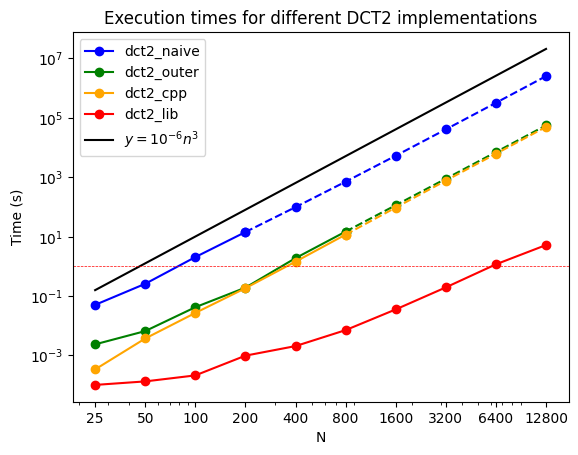
\includegraphics[width=0.5\textwidth]{images/times_plot.png}
        \caption{Risultato del benchmark su scala logaritmica (i \textit{tempi tratteggiati} sono solo stimati)}
        \label{fig:times_plot}
    \end{figure}

    Dal grafico \ref{fig:times_plot} si nota come i risultati della sperimentazione confermino l'attesa teorica di una \textbf{complessità temporale} $T(n) = \theta(n^3)$ per le implementazioni \textit{custom}, mentre l'implementazione \textit{fast} della libreria mostra una capacità di scalare decisamente superiore, sebbene non sia immediato riconoscere l'andamento asintotico. 
    
    Confrontando invece solo le tre versioni \textit{custom}, risulta evidente che, a parità di complessità computazionale, le implementazioni \textbf{\textit{dct\_outer}} e \textbf{\textit{dct\_cpp}} siano nettamente superiori a \textbf{\textit{dct\_naive}}, al punto da riuscire a trattare matrici \textit{16 volte più grandi} con tempi dagli \textit{stessi ordini di grandezza}.

    Inoltre, si evince come sia possibile ottenere ottime prestazioni da un linguaggio di programmazione \textit{interpretato}, orientato alla \textit{portabilità} e alla \textit{semplicità di utilizzo} come \textbf{python}: nonostante i limiti dovuti alla sua struttura, è possibile raggiungere prestazioni molto vicine a quelle del \textbf{C/C++}, a patto di fare ampio utilizzo di librerie specializzate ed efficienti (e sviluppate in linguaggi performanti) come \textbf{\textit{numpy}} (sviluppata in C). 